\documentclass[a4paper]{report}

\usepackage[latin1]{inputenc} % accents
\usepackage[T1]{fontenc}      % caract�res fran�ais
\usepackage[francais]{babel}  % langue
\usepackage{graphicx}         % images
\usepackage{verbatim}         % texte pr�format�
\usepackage{listings}
\usepackage[]{algorithm2e}
\usepackage[margin=0.8in]{geometry}
\usepackage[table]{xcolor}
\usepackage{xcolor}
\usepackage{hyperref}
\usepackage{color}

\definecolor{mygreen}{rgb}{0,0.6,0}
\definecolor{mygray}{rgb}{0.5,0.5,0.5}
\definecolor{mymauve}{rgb}{0.58,0,0.82}

\lstset{ %
  backgroundcolor=\color{white},   % choose the background color; you must add \usepackage{color} or \usepackage{xcolor}
  basicstyle=\footnotesize,        % the size of the fonts that are used for the code
  breakatwhitespace=false,         % sets if automatic breaks should only happen at whitespace
  breaklines=true,                 % sets automatic line breaking
  captionpos=b,                    % sets the caption-position to bottom
  commentstyle=\color{mygreen},    % comment style
  deletekeywords={...},            % if you want to delete keywords from the given language
  escapeinside={\%*}{*)},          % if you want to add LaTeX within your code
  extendedchars=true,              % lets you use non-ASCII characters; for 8-bits encodings only, does not work with UTF-8
  frame=single,	                   % adds a frame around the code
  keepspaces=true,                 % keeps spaces in text, useful for keeping indentation of code (possibly needs columns=flexible)
  keywordstyle=\color{blue},       % keyword style
  language=Octave,                 % the language of the code
  otherkeywords={*,...},            % if you want to add more keywords to the set
  numbers=left,                    % where to put the line-numbers; possible values are (none, left, right)
  numbersep=5pt,                   % how far the line-numbers are from the code
  numberstyle=\tiny\color{mygray}, % the style that is used for the line-numbers
  rulecolor=\color{black},         % if not set, the frame-color may be changed on line-breaks within not-black text (e.g. comments (green here))
  showspaces=false,                % show spaces everywhere adding particular underscores; it overrides 'showstringspaces'
  showstringspaces=false,          % underline spaces within strings only
  showtabs=false,                  % show tabs within strings adding particular underscores
  stepnumber=2,                    % the step between two line-numbers. If it's 1, each line will be numbered
  stringstyle=\color{mymauve},     % string literal style
  tabsize=2,	                   % sets default tabsize to 2 spaces
  title=\lstname                   % show the filename of files included with \lstinputlisting; also try caption instead of title
}

\lstdefinestyle{customc}{
  belowcaptionskip=1\baselineskip,
  breaklines=true,
  frame=L,
  xleftmargin=\parindent,
  language=C,
  showstringspaces=false,
  basicstyle=\footnotesize\ttfamily,
  keywordstyle=\bfseries\color{green!40!black},
  commentstyle=\itshape\color{purple!40!black},
  identifierstyle=\color{blue},
  stringstyle=\color{orange},
}

\lstset{escapechar=@,style=customc}

\lstdefinestyle{DOS}
{
    backgroundcolor=\color{black},
    basicstyle=\scriptsize\color{white}\ttfamily
}

\addto\captionsfrancais{% Replace "english" with the language you use
  \renewcommand{\contentsname}%
    {Sommaire}%
}

\begin{document}

\begin{titlepage}
\fontfamily{phv}\selectfont
\vspace*{\stretch{1}}
\begin{flushright}\LARGE
Security bugtracker
\end{flushright}
\hrule
\begin{flushleft}\huge\bfseries
User Manual
\end
{flushleft}
\vspace*{\stretch{2}}
\begin{center}
Eric Therond
\end{center}
\end{titlepage}

\tableofcontents

\chapter{Installation}

  \section{Overview}

\textit{Security-bugtracker} is a tool based on three dependencies at this time :
\begin{itemize}
\item webissues : http://webissues.mimec.org/
\item openvas : http://www.openvas.org/
\item dependency-check : https://github.com/jeremylong/DependencyCheck
\end{itemize}
\vspace{5mm}
Each of this tool can be installed on different or same server.
\vspace{5mm}
\begin{center}
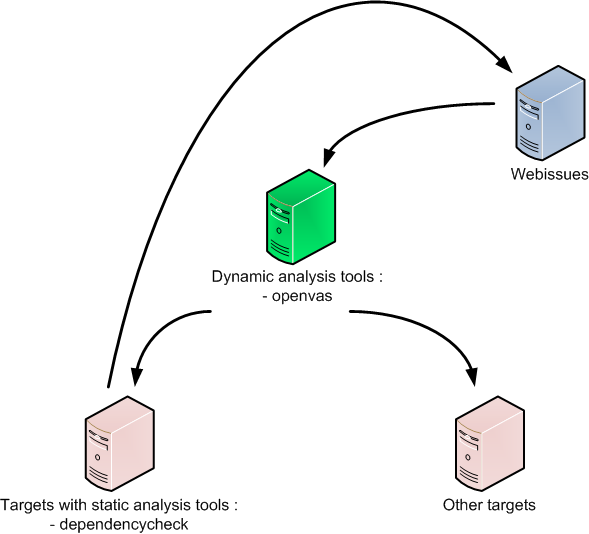
\includegraphics[scale=0.60]{sec1.png}
\vspace{5mm}
\end{center}
  \newpage
  
  \section{Openvas}
See the documentation on the official web site : http://www.openvas.org/install-source.html\\
On the same server install a web server and php, then copy the following module of this project :\\
/security-bugtracker/security\_tools/openvas\\
Then edit /security-bugracker/security\_tools/openvas/openvas.conf.php :\\
\begin{lstlisting}[style=customc]
<?php

$CONF_WS_OPENVAS_LOGIN = "test";
$CONF_WS_OPENVAS_PASSWORD = "test";
$CONF_WEBISSUES_OPENVAS_LOGIN = "openvas";
$CONF_WEBISSUES_OPENVAS_PASSWORD = "openvas";
$CONF_WEBISSUES_WS_ENDPOINT = "http://localhost:8080/webissues-server-1.1.4/client/webservices.php";
$CONF_OPENVAS_ALERT_URL = "http://localhost:8080/webissues-server-1.1.4/client/security_tools/openvas.php";
$CONF_OPENVAS_ADMIN_LOGIN = "admin";
$CONF_OPENVAS_ADMIN_PASSWORD = "0825839c-0d3f-4417-a118-954a78e2553c";
$CONF_OPENVAS_CONFIG_ID = "a0e8fed8-45c1-4890-bd08-671257f63308";
$CONF_OPENVAS_PATH_OMP = "/usr/local/bin/omp";

?>
\end{lstlisting}\
\begin{itemize}
\item CONF\_WS\_OPENVAS\_LOGIN
\item CONF\_WS\_OPENVAS\_PASSWORD
\end{itemize}
are the credentials for this module.
\vspace{5mm}
\begin{itemize}
\item CONF\_WEBISSUES\_OPENVAS\_LOGIN
\item CONF\_WEBISSUES\_OPENVAS\_PASSWORD
\item CONF\_WEBISSUES\_WS\_ENDPOINT
\end{itemize}
 will be completed later.
\vspace{5mm}
\begin{itemize}
\item CONF\_OPENVAS\_ALERT\_URL
\end{itemize}
 is the address of this module on this web server.
\vspace{5mm}
\begin{itemize}
\item CONF\_OPENVAS\_ADMIN\_LOGIN
\item CONF\_OPENVAS\_ADMIN\_PASSWORD
\end{itemize}
 are the openvas admin credentials.
\vspace{5mm}
\begin{itemize}
\item CONF\_OPENVAS\_CONFIG\_ID
\end{itemize}
is the default config id for run a scan with openvas, check your config with this openvas command
\vspace{5mm}
\begin{lstlisting}[style=DOS]
linux-3ig5:/home/eric/security-bugracker/documentation # omp -u admin -w 0825839c-0d3f-4417-a118-954a78e2553c -p 9393 --get-configs
8715c877-47a0-438d-98a3-27c7a6ab2196  Discovery
085569ce-73ed-11df-83c3-002264764cea  empty
daba56c8-73ec-11df-a475-002264764cea  Full and fast
698f691e-7489-11df-9d8c-002264764cea  Full and fast ultimate
708f25c4-7489-11df-8094-002264764cea  Full and very deep
a0e8fed8-45c1-4890-bd08-671257f63308  Full and very deep Clone 1
74db13d6-7489-11df-91b9-002264764cea  Full and very deep ultimate
2d3f051c-55ba-11e3-bf43-406186ea4fc5  Host Discovery
bbca7412-a950-11e3-9109-406186ea4fc5  System Discovery
\end{lstlisting}
\vspace{5mm}
\begin{itemize}
\item CONF\_OPENVAS\_PATH\_OMP
\end{itemize}
is the path of your omp binary on this server.
  \newpage

  \section{Dependency-check}
See the documentation on the official web site : https://github.com/jeremylong/DependencyCheck
  
  \section{Webissues}
See the documentation on the official web site : http://wiki.mimec.org/wiki/WebIssues/Installation\\
Once the bugtracker is installed, copy the following module of this project to your webissues root directory :\\
/security-bugracker/webissues-server-1.1.4\\
Next go at this address (replace the name, port, path with rights information on your server) :\\
http://localhost:8080/webissues-server-1.1.4/client/securityplugin.php
\newline
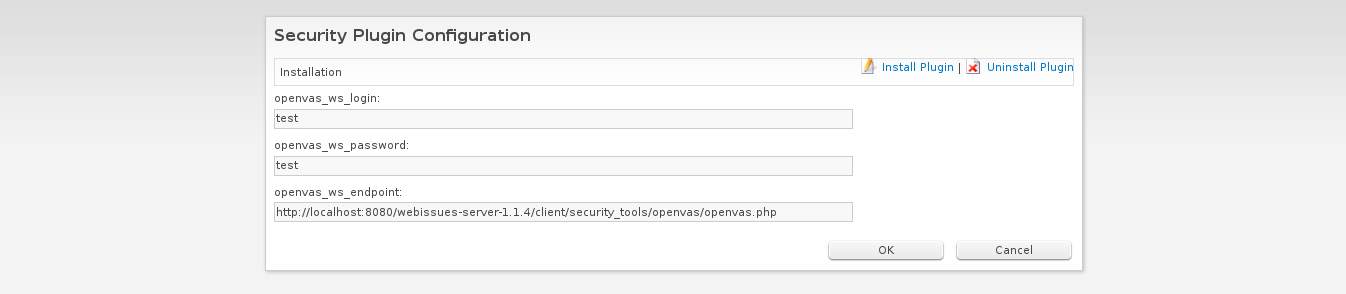
\includegraphics[scale=0.50]{sec2.png}
\vspace{5mm}
\newline
select install plugin and enter choosen values when the openvas module was installed above :\\
\begin{itemize}
\item CONF\_WS\_OPENVAS\_LOGIN
\item CONF\_WS\_OPENVAS\_PASSWORD
\item CONF\_OPENVAS\_ALERT\_URL
\end{itemize}
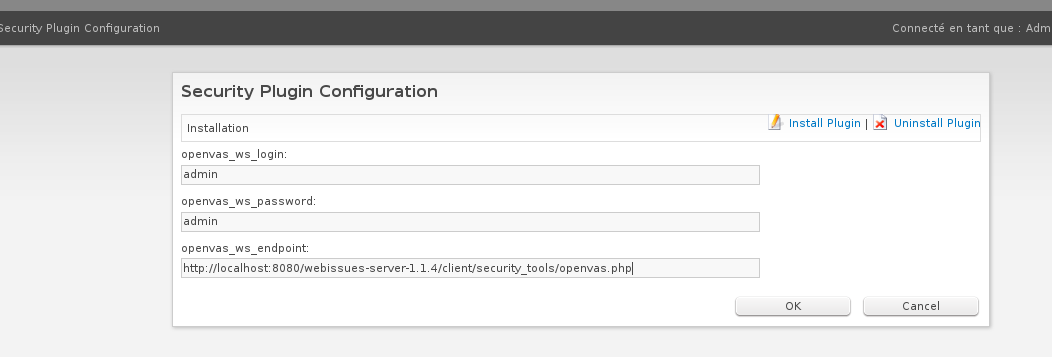
\includegraphics[scale=0.50]{sec3.png}
\vspace{5mm}
\newline
Now create a new openvas user on webissues.
\chapter{Use}

  \section{add a project}
\textbf{Don't forget to use basic authentification with a login which have the good rights on webissues when using the webservices}.\\
Add a project with the following web service method or via the traditional him of web issues :
\begin{lstlisting}[style=customc]
<soapenv:Envelope xmlns:soapenv="http://schemas.xmlsoap.org/soap/envelope/" xmlns:v1="http://securitybugtracker/V1">
   <soapenv:Header/>
   <soapenv:Body>
      <v1:addproject>
         <name>TEST</name>
         <description>TEST</description>
      </v1:addproject>
   </soapenv:Body>
</soapenv:Envelope>
\end{lstlisting}
\begin{lstlisting}[style=customc]
<SOAP-ENV:Envelope xmlns:SOAP-ENV="http://schemas.xmlsoap.org/soap/envelope/" xmlns:ns1="http://securitybugtracker/V1">
   <SOAP-ENV:Body>
      <ns1:addproject_Response>
         <id_details>
            <id_project>29</id_project>
            <id_folder_bugs>81</id_folder_bugs>
            <id_folder_servers>82</id_folder_servers>
            <id_folder_codes>83</id_folder_codes>
            <id_folder_scans>84</id_folder_scans>
         </id_details>
      </ns1:addproject_Response>
   </SOAP-ENV:Body>
</SOAP-ENV:Envelope>
\end{lstlisting}
  \section{add a member}
  Add a member for this project (the openvas account created during the installation) :
\begin{lstlisting}[style=customc]
<soapenv:Envelope xmlns:soapenv="http://schemas.xmlsoap.org/soap/envelope/" xmlns:v1="http://securitybugtracker/V1">
   <soapenv:Header/>
   <soapenv:Body>
      <v1:addmember>
         <id_user>4</id_user>
         <id_project>29</id_project>
         <access>admin</access>
      </v1:addmember>
   </soapenv:Body>
</soapenv:Envelope>
\end{lstlisting}
\begin{lstlisting}[style=customc]
<SOAP-ENV:Envelope xmlns:SOAP-ENV="http://schemas.xmlsoap.org/soap/envelope/" xmlns:ns1="http://securitybugtracker/V1">
   <SOAP-ENV:Body>
      <ns1:addmember_Response>
         <result_details>
            <result>true</result>
         </result_details>
      </ns1:addmember_Response>
   </SOAP-ENV:Body>
</SOAP-ENV:Envelope>
\end{lstlisting}
  
  \section{add a server}
  Add a target server for this project :
\begin{lstlisting}[style=customc]
<soapenv:Envelope xmlns:soapenv="http://schemas.xmlsoap.org/soap/envelope/" xmlns:v1="http://securitybugtracker/V1">
   <soapenv:Header/>
   <soapenv:Body>
      <v1:addserver>
         <id_folder_servers>82</id_folder_servers>
         <hostname>eric-pc</hostname>
         <description>eric-pc</description>
         <use>Production</use>
         <ipsaddress>127.0.0.1</ipsaddress>
      </v1:addserver>
   </soapenv:Body>
</soapenv:Envelope>
\end{lstlisting}
\begin{lstlisting}[style=customc]
<SOAP-ENV:Envelope xmlns:SOAP-ENV="http://schemas.xmlsoap.org/soap/envelope/" xmlns:ns1="http://securitybugtracker/V1">
   <SOAP-ENV:Body>
      <ns1:addserver_Response>
         <result_addserver_details>
            <id_server>1676</id_server>
         </result_addserver_details>
      </ns1:addserver_Response>
   </SOAP-ENV:Body>
</SOAP-ENV:Envelope>
\end{lstlisting}
  
  \section{add a code}
  Add a target code path for this project :
\begin{lstlisting}[style=customc]
<soapenv:Envelope xmlns:soapenv="http://schemas.xmlsoap.org/soap/envelope/" xmlns:v1="http://securitybugtracker/V1">
   <soapenv:Header/>
   <soapenv:Body>
      <v1:addcode>
         <id_folder_codes>83</id_folder_codes>
         <name>java test</name>
         <description>java tes</description>
         <code>/home/eric/test/libs-java</code>
      </v1:addcode>
   </soapenv:Body>
</soapenv:Envelope>
\end{lstlisting}
\begin{lstlisting}[style=customc]
<SOAP-ENV:Envelope xmlns:SOAP-ENV="http://schemas.xmlsoap.org/soap/envelope/" xmlns:ns1="http://securitybugtracker/V1">
   <SOAP-ENV:Body>
      <ns1:addcode_Response>
         <result_addcode_details>
            <id_code>1680</id_code>
         </result_addcode_details>
      </ns1:addcode_Response>
   </SOAP-ENV:Body>
</SOAP-ENV:Envelope>
\end{lstlisting}

  \section{scan the targets}
  \subsection{Dynamic scan with openvas}
\begin{lstlisting}[style=customc]
<soapenv:Envelope xmlns:soapenv="http://schemas.xmlsoap.org/soap/envelope/" xmlns:v1="http://securitybugtracker/V1">
   <soapenv:Header/>
   <soapenv:Body>
      <v1:addcode>
         <id_folder_codes>83</id_folder_codes>
         <name>java test</name>
         <description>java tes</description>
         <code>/home/eric/test/libs-java</code>
      </v1:addcode>
   </soapenv:Body>
</soapenv:Envelope>
\end{lstlisting}
\begin{lstlisting}[style=customc]
<SOAP-ENV:Envelope xmlns:SOAP-ENV="http://schemas.xmlsoap.org/soap/envelope/" xmlns:ns1="http://securitybugtracker/V1">
   <SOAP-ENV:Body>
      <ns1:addcode_Response>
         <result_addcode_details>
            <id_code>1680</id_code>
         </result_addcode_details>
      </ns1:addcode_Response>
   </SOAP-ENV:Body>
</SOAP-ENV:Envelope>
\end{lstlisting}

  \section{Results}
You can view the results of your precedings actions with th him of webissues :
\newline
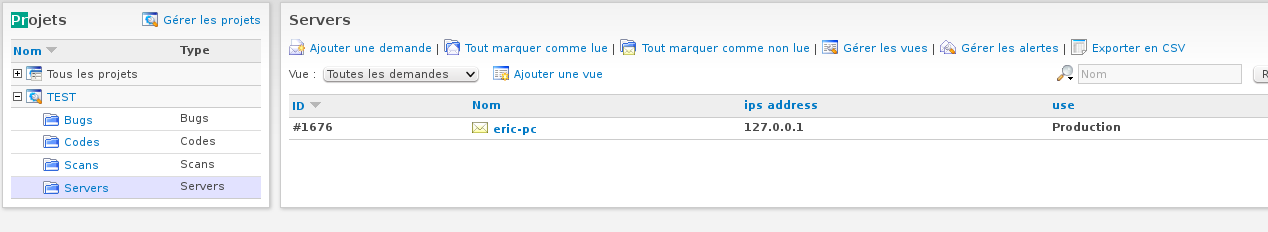
\includegraphics[scale=0.50]{sec4.png}
\vspace{5mm}
\newline
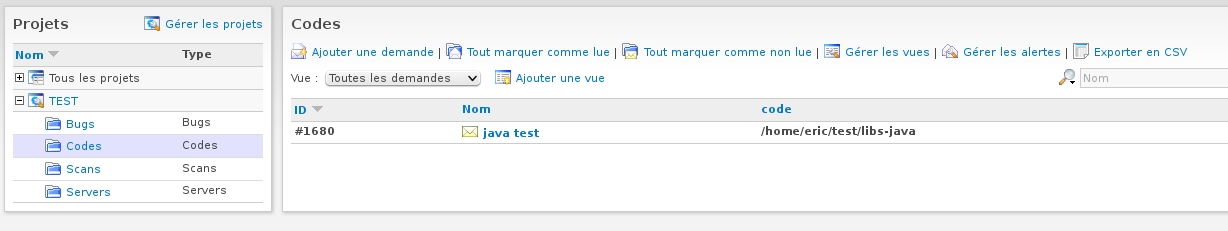
\includegraphics[scale=0.50]{sec5.png}
\vspace{5mm}
\newline
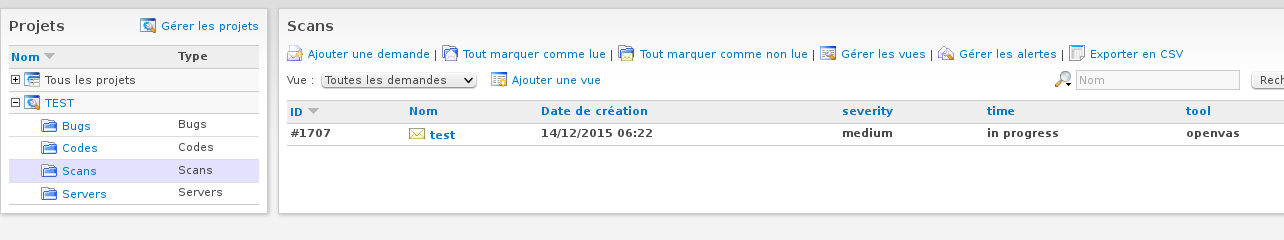
\includegraphics[scale=0.50]{sec6.png}
\vspace{5mm}
\newline
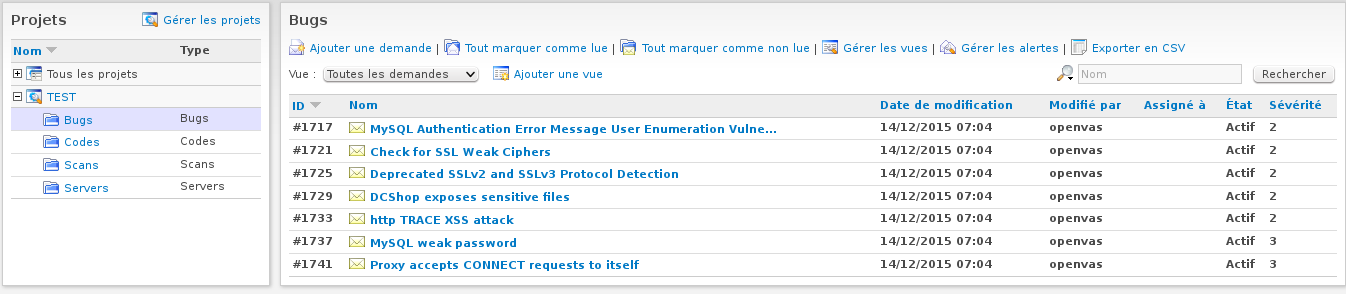
\includegraphics[scale=0.50]{sec7.png}
\vspace{5mm}
\newline

% \listoffigures
% \listoftables

\end{document}
